\pagestyle{fancy}
\chapter{Experimental methods}
\label{Chap2}
    
    Tools and experimental methods provide the ways to make structures. In this part we will see how the devices and methods used for the process work. In the last part we will talk about the dilution cryostat which was used to cool down samples.

    \section{Resists}
        
        The first part of the process is the deposition of resists on a Silicon wafer with a layer of SiO$_2$.

The resists we use consists of polymer materials : Polymethyl Methacrilate (PMMA) and Methyl Methacrilate (MMA) (See Appendix \ref{appendixresists} Fig. \ref{PMMA}). PMMA is a polymer made out of MMA.
            We depose the resists on the top of the wafer and then a spinner rotates the wafer and makes a thin and uniform layer of resist, with a thickness from 100nm to 500 nm depending on the rotation speed and the type of the resist. In our case, the copolymer thickness is around 400nm.
            
            \begin{figure}
                \centering
                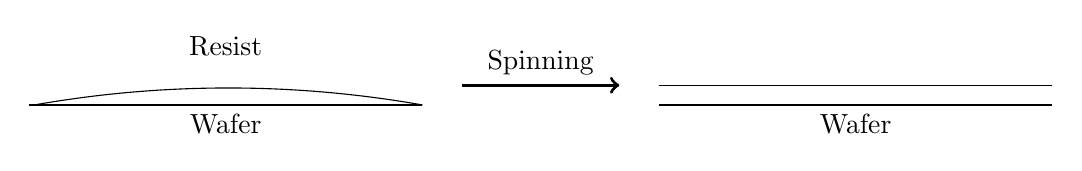
\begin{tikzpicture}
                    \draw [thick] (0,0)--(5,0);
                    \draw (5,0) arc(80:100:14.2);
                    \draw [->, very thick] (5.5,0.25)--(7.5,0.25)node[midway,above]{Spinning};
                    \draw [thick](8,0)--(13,0);
                    \draw (8,0.25)--(13,0.25);
                    \draw (2.5,0)node[below]{Wafer};
                    \draw (10.5,0)node[below]{Wafer};
                    \draw (2.5,0.5)node[above]{Resist};
                \end{tikzpicture}
                \caption{Spinning + Baking}
            \end{figure}
                   
            Practically, we use these two types of resists because they have a different reactivity to the e-beam lithography and to the development process. These two layers have different thicknesses since they do nothave the same role. PMMA acts as a pattern designer, so it cans be thin ($\sim$ 100 - 200nm), whereas we will dig the MMA to create undercuts where the metal will be deposed in the evaporator, this is why the MMA layer needs to be thicker ($\sim$ 1.2$\mu$m), to avoid evaporating on the undercut. 
         Then the resists are baked with a hot plate. The datasheet of the resists can be find in Ref. \cite{Datasheet}. We finally obtain the cross-section shown in Fig. \ref{resine}.
            
            \begin{figure}
                \centering 
                \begin{tikzpicture}
                    \draw (0,0)--(10,0);
                    \draw (5,-0.5) node{Wafer $Si/SiO_2$};
                    \draw (0,2)--(10,2);
                    \draw (5,1)node{MMA};
                    \draw (0,2.5)--(10,2.5);
                    \draw (5,2.25) node{PMMA};
                \end{tikzpicture}
                \caption{Cross-section view after resist deposit, spinning and baking}
                \label{resine}
            \end{figure}
            
                        
            The resists we use are sensitive to electrons with a particular energy, what we will do next is to expose the resist to an electron beam (See \ref{explicationebl}) which will imply structural modifications. The electrons break the polymer into smaller pieces, which make the exposed resist more soluble in Methyl IsoButyl Ketone (MIBK) (See \ref{development}).
            
              Other type of resists exists, especially some resists damaged by light (photoresits), which are mostly used for semiconductors-based structures.
              
    \section{Electron Beam Lithography and development}
        
        Once the wafer have been prepared and is covered by resists, we can draw a pattern in these resists, with the Electron Beam Lithography (EBL).
        
        \subsection{Electron Beam Lithography}
            The EBL is a tool which is used to design the patterns we want to have for our structures\cite{EBL_theory}. It sends an electron beam onto the resist to damage the bonds of the resist, making the exposed area sensitive to the development process. The functionnal diagram can be found in Appendix \ref{appendixEBL} Fig. \ref{EBLschema}.The E-beam lithography gives the opportunity to make very small structures, down to few tens of nanometer in size with a resolution of few nanometers. The drawback of such low resolution is the writing time, a compromise between good accuracy and reasonable writing time has thus to be found.
            
            For example, the only part that requires an good accuracy in our process is the junction, so we have to use a good resolution there, but for the leads, which are much larger when the actual size does not matter, so we can choose to go faster. 
            In addition to the primary electrons from the beam, the resist is also affected by the secondary elestrons, backscattered from the substrate. These electrons will create a wider exposed area below the PMMA and is called "undercut" (See Fig. \ref{waferEBL}). This is this undercut that give the possibility to shadow evaporation (see below).
            
            \label{explicationebl}
                    
            \begin{figure}
                \centering
                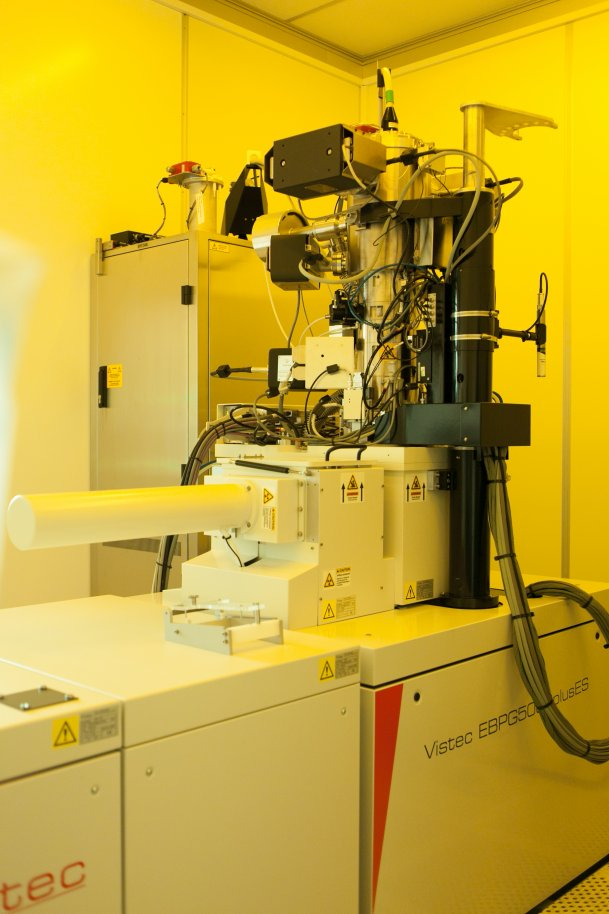
\includegraphics[width=100pt]{EBL.jpg}
                \caption{Electron Beam Lithographier Vistec of Micronova cleanroom}
            \end{figure}
            
            Once the wafer has been exposed, it can be represented by Fig \ref{waferEBL}.
                    
            \begin{figure}
                \centering
                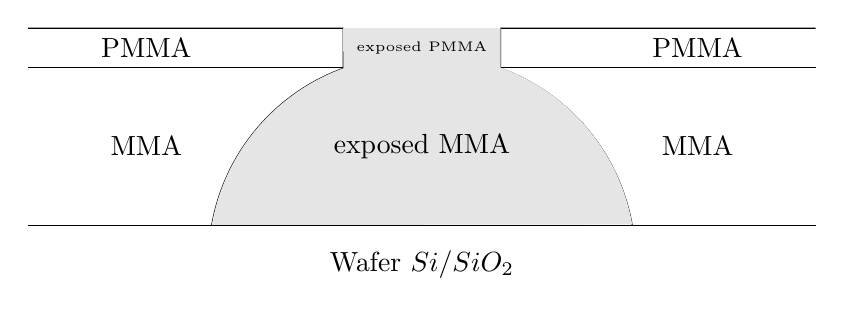
\begin{tikzpicture}
                \draw (0,0)--(10,0);
                \draw (5,-0.5) node{Wafer $Si/SiO_2$};
                \draw (2.33,0) arc(170:110:2.6)--(4,2.5)--(0,2.5);
                \draw (7.67,0) arc(10:70:2.6)--(6,2.5)--(10,2.5);
                \fill [color=gray!20](2.33,0) arc(170:110:2.6)--(4,2.5)--(6,2.5)--(6,2) arc(70:10:2.6);
                \draw (0,2)--(4,2);
                \draw (6,2)--(10,2);
                \draw (1.5,1) node{MMA};
                \draw (8.5,1) node{MMA};
                \draw (1.5,2.25) node{PMMA};
                \draw (8.5,2.25) node{PMMA};
                \draw (5,2.25)node{{\tiny exposed PMMA}};
                 \draw (0,0)--(10,0);
                \draw (5,1)node{exposed MMA};
                \end{tikzpicture}
                \caption{Cross-section view after EBL}
                \label{waferEBL}
            \end{figure}
        
        \subsection{Development}
        
            \label{development}
            The Development consists in the withdrawal of the exposed resit. It is realized by chemical reactions.
            
            
            %Our goal is to make junction between Al and Cu, if we depose Al or Cu on this wafer, they will depose everywhere and we will just have Aluminium covered by Copper. To make a junction, we need a way to not depose metal everywhere. This is the role of the undercuts and evaporation angles (See \ref{evapangles}).
            
            The MIBK(See Appendix \ref{appendixresists} Fig. \ref{MIBK}) will dissolve fastly the exposed PMMA and MMA (Fig. \ref{aprèsMIBK}).If we want to increase the width of the undercut, it is possible to add an extra step and to use MethylGlycol after the development in MIBK. The MethyGlycol can dissolve MMA and thus increase the undercut \cite{methylglycol}. This is particularly useful if we want to work with large angles.
            
            There, we can see that if we depose metal with a certain angle, they will overlap only in the chosen area. Finally, we dive the sample in Isopropanol to stop the reaction.

The dissolution will depend on the time we dive the samples into the chemicals, we need to chose this time considering the width of the undercuts but ensure that PMMA does not collapse.
            
            \begin{figure}
                \centering
                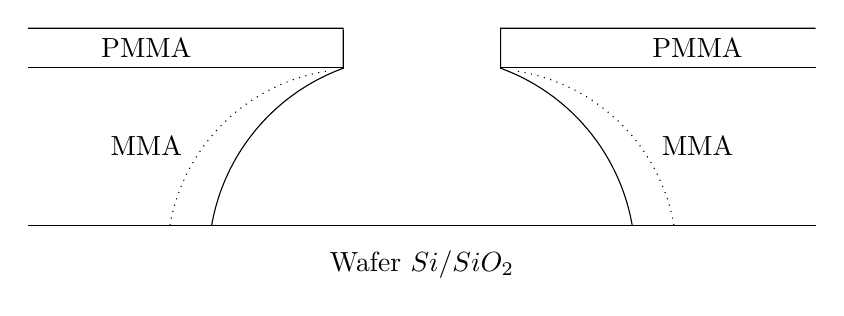
\begin{tikzpicture}
                \draw (0,0)--(10,0);
                \draw (5,-0.5) node{Wafer $Si/SiO_2$};
                \draw (2.33,0) arc(170:110:2.6)--(4,2.5)--(0,2.5);
                \draw (7.67,0) arc(10:70:2.6)--(6,2.5)--(10,2.5);
                \draw [dotted](1.8,0) arc(170:98:2.4);
                \draw [dotted] (8.2,0) arc(10:82:2.4);
                \draw (0,2)--(4,2);
                \draw (6,2)--(10,2);
                \draw (1.5,1) node{MMA};
                \draw (8.5,1) node{MMA};
                \draw (1.5,2.25) node{PMMA};
                \draw (8.5,2.25) node{PMMA};
                \end{tikzpicture}
                \caption{Cross-section view after MIBK (full lines), and after MethyGlycol (dotted lines)}
                \label{aprèsMIBK}
            \end{figure}
            
    \section{Evaporation}
        During the evaporation step, we make the junctions by evaporating metal.
        
        \subsection{Functioning of evaporator}
        
        The evaporator is a tool that allows to deposit a uniform, thin layer of metal. A filament is submitted to a large tension (10kV) and current, it emits electrons that are deflected with a magnetic field to focus on a crucible which contains metal. The metal will melt, or even sublimate, depending on the metal. The atoms can move without collision in the very low pressure chamber ($P\sim10^{-7}mbar$) : the mean free path is longer ($\sim$ 1km) than the distance between the crucible and the sample holder ($\sim$ 50cm). The deposition of the atoms is very uniform and the thickness is measured with capacitive sensors.
        The chamber of the evaporator is connected to a pure Oxygen line, in order to perform oxidation \textit{in situ}. The most common superconductor used is Al, and its oxidation is very rapid (an exposure of 2mbar of O$_2$ during 2 minutes is enough to create a tunnel barrier).
        
        \subsection{The Plasma gun}
        
        The evaporator is also equipped with a Plasma Gun, with Argon valve. The plasma is mostly used at low power to ease the lift-off (See \ref{lift-off}) by weakening the resist and to clean the surface. But with the accurate parameters it can also be used for etching. The idea of plasma etching is to etch native oxide of a material, which has been grown in another process, so exposed to air, and to make contact in a controlled way (clean contact or tunnel barrier).
        
        %One of the goals of this project is to characterize this technique in the evaporator here : characterize the plasma and determine its effect on samples (See \ref{Chap3}). We need to know better about plasma etching because the nanowires will come from Copenhaguen and the Aluminium layer will be strongly oxidized, thing that we do not want. We will need to get rid of it one way or another, this is why we try plasma etching. We will realize different junctions with different plasma parameters to know better how it behaves.         
            
            \begin{figure}
                \centering
                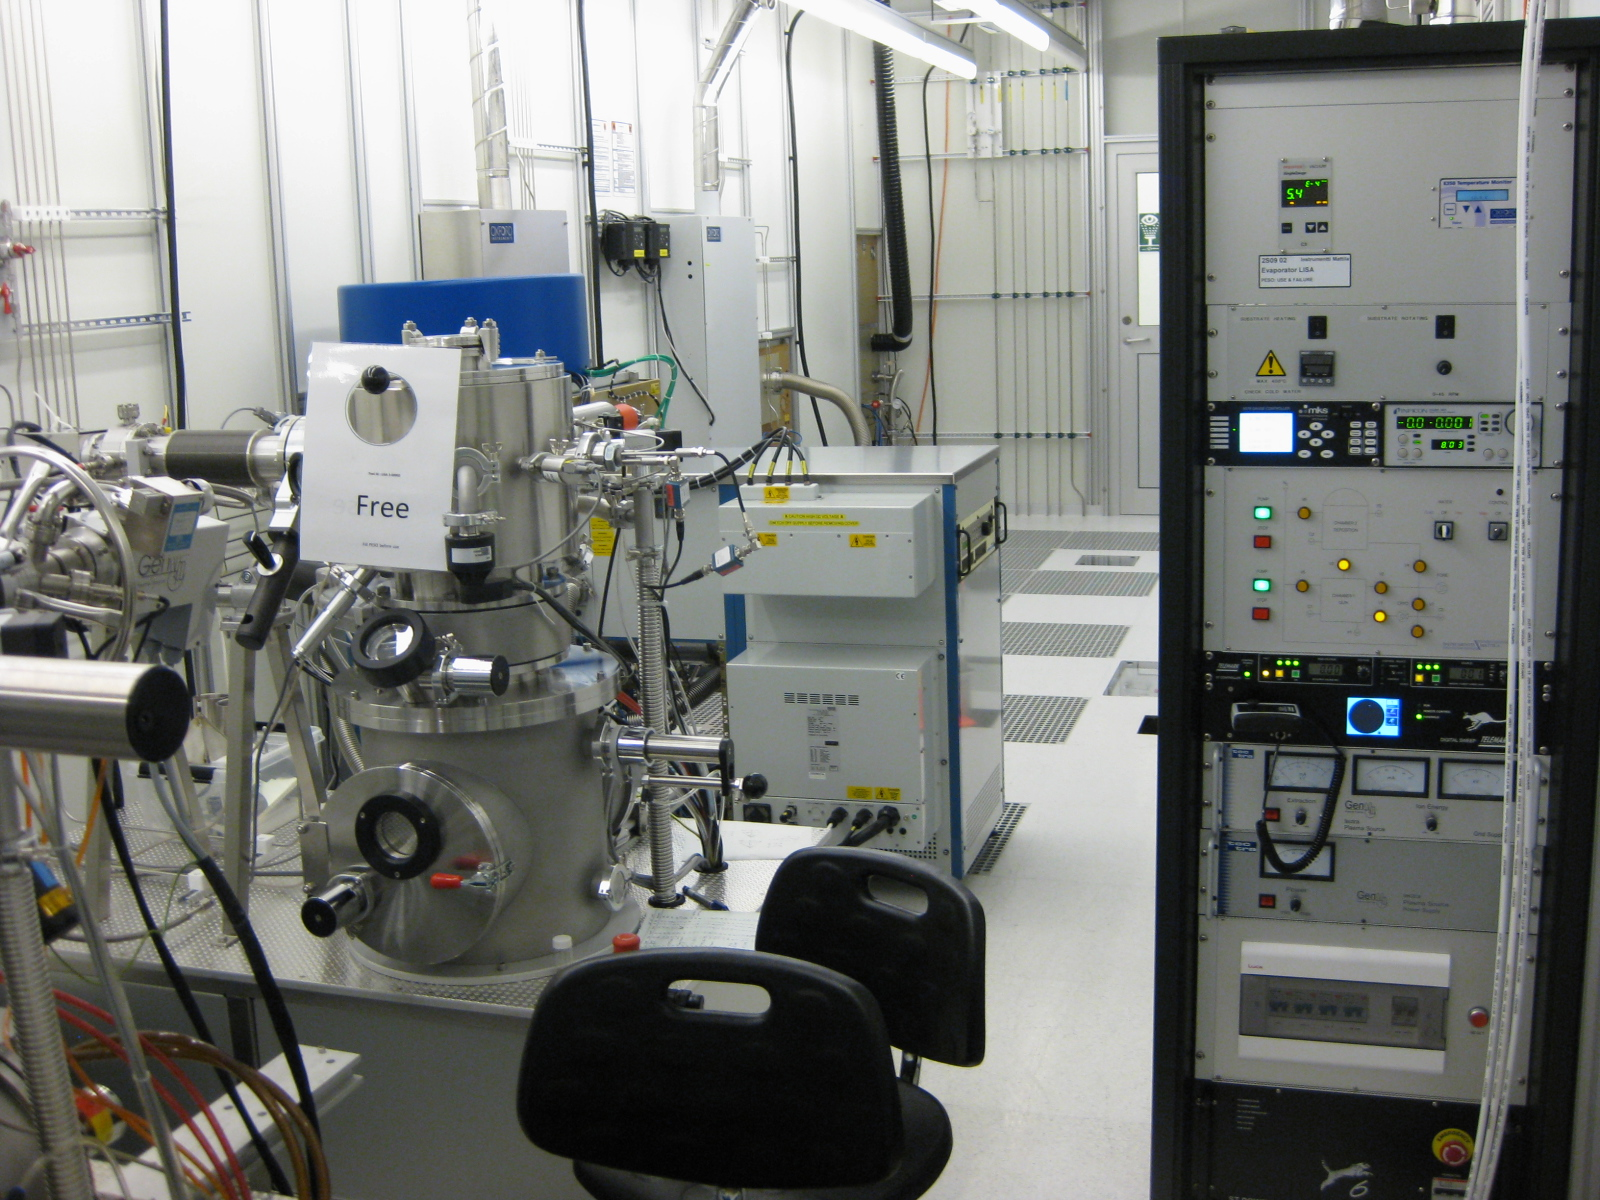
\includegraphics[width=200pt]{LISA.JPG}
                \caption{Picture of the LISA evaporator in Micronova cleanroom}
            \end{figure}
            
            
            \subsection{Evaporator in action}
            
                \label{evapangles}
                The Fig. \ref{evaporation} shows the principle of evaporation. First, we depose the first layer of metal with a previously determined angle. If needed, it is possible to oxidize to obtain a tunnel barrier, then another layer is evaporated, with another angle. The pattern and the angles are such that only the active parts (the junctions) will overlap. Thus, we can see that even it they are in the same undercut, they do not touch each other. To make the junction, we have to have two different undercuts that overlap.
                
            \begin{figure}
            \centering
            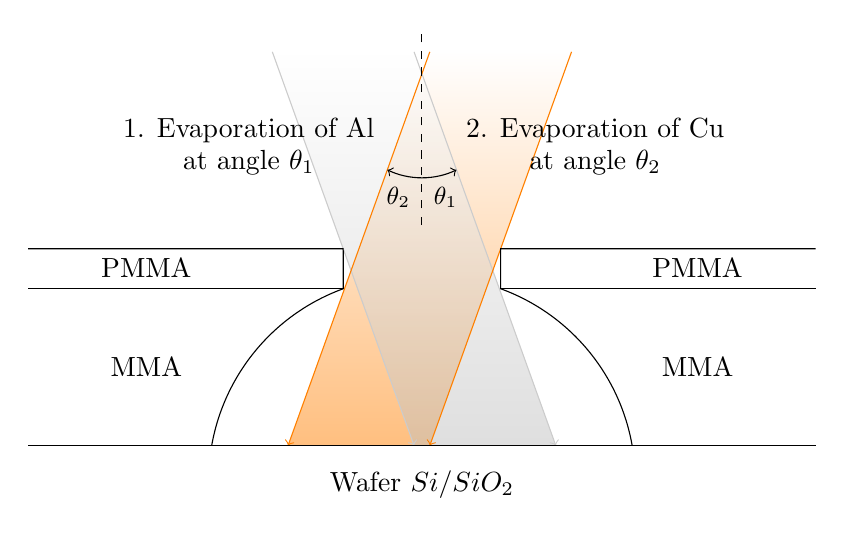
\begin{tikzpicture}
                
                \shadedraw[bottom color=orange,top color=white, draw=orange, fill opacity=0.5,draw opacity=0](5.1,5)--(3.3,0)--(5.1,0)--(6.9,5)-- cycle;
                \shadedraw[bottom color=gray!50,top color=white, draw=gray!40, fill opacity=0.5, draw opacity=0](4.9,5)--(6.7,0)--(4.9,0)--(3.1,5)--cycle;   
                \draw [color=gray!40,->] (4.9,5)--(6.7,0);
                \draw [color=gray!40,->] (3.1,5)--(4.9,0);  
                \draw [color=orange,->] (5.1,5)--(3.3,0);
                \draw [color=orange,<-] (5.1,0)--(6.9,5);
                          
                \draw (0,0)--(10,0);
                \draw (5,-0.5) node{Wafer $Si/SiO_2$};
                \draw (2.33,0) arc(170:110:2.6)--(4,2.5)--(0,2.5);
                \draw (7.67,0) arc(10:70:2.6)--(6,2.5)--(10,2.5);
                \draw (0,2)--(4,2);
                \draw (6,2)--(10,2);
                \draw (1.5,1) node{MMA};
                \draw (8.5,1) node{MMA};
                \draw (1.5,2.25) node{PMMA};
                \draw (8.5,2.25) node{PMMA};
                \draw [dashed](5,2.8)--(5,5.3);
                \draw [->] (5,3.4) arc(-90:-116:1);
                \draw (2.8,4) node{1. Evaporation of Al};
                \draw(2.8,3.6) node{at angle $\theta_1$} ;               
                \draw (4.7,3.4)node[below]{{\small $\theta_2$}};
                \draw [->] (5,3.4) arc(-90:-64:1);
                \draw (7.2,4)node {2. Evaporation of Cu};
                \draw (7.2,3.6)node{at angle $\theta_2$};
                \draw (5.3,3.4)node[below]{{\small $\theta_1$}};
                
            \end{tikzpicture} 
            \caption[Cross-section during evaporation]{Cross-section during evaporation (the two metal are evaporated succesively, not at the same time)}
            \label{evaporation}
            \end{figure}
        
                
                
                
    \section{Lift-off and Scanning Electron Microscope}

        \subsection{Lift-off : resist withdrawal}
        \label{lift-off}
        
            The lift-off is a process where the resist is removed to get our final structures. The chip is dived into an acetone bath, which will dissolve the resist and left on the substrate only the device made.
            
        \subsection{Scanning Electron Microscope}
            The functioning of Scanning Electron Microscope (SEM) is very similar to the EBL one, since actually, SEM and EBL are the same instrument, except that this time we do not want to weaken the matter but to observe the scattering of electrons within it. This allows us to check if the junctions made looks measureable, if metals evaporated overlap in the chosen area, meaning that the angle is correct. It is useful for a process that is not completely established, where the angles, or the EBL electron dose are still to be improved.
            
            \begin{figure}
                \centering
                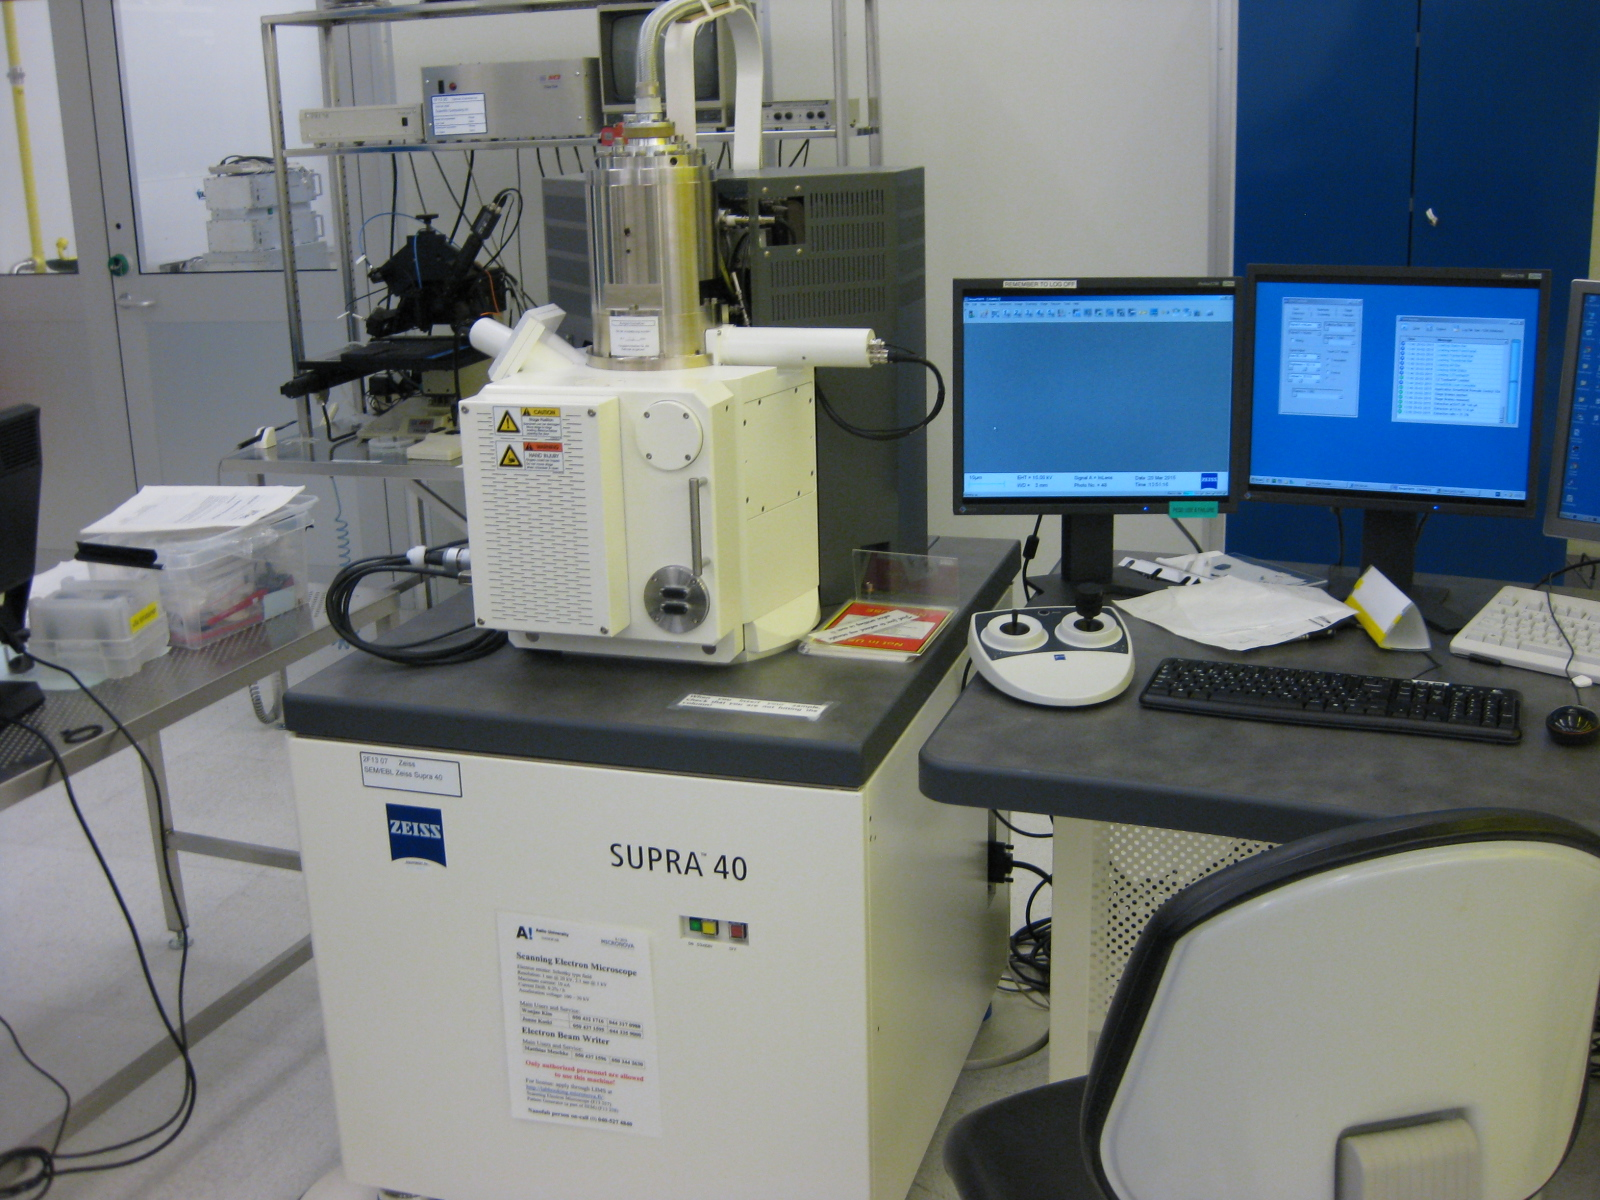
\includegraphics[width=200pt]{SEM.JPG}
                \caption{Scanning Electron Microscope}
            \end{figure}
            
        \subsection{Observation of the samples}
            The SEM is very similar to an optical microscope, in the way that the clarity of the image will depend on the focusing of the beam on the sample, except that it is not light here but electrons. This can be problematic as it can be possible to charge the objects observed if the beam stays too long on the same spot, and this can damage the junctions, especially if they are small.
            
            As in the EBL, the matter scatters the electron, especially metals. These scattered electrons can be detected with the secondary electron mode. Since each metal scatters electrons in a different way, in this mode will only the metals appear and different contrasts allow to distinguish them, despiting the brightness and quality of the signal (few scattered electrons inducing noise).
            
            %requires some adjustments in order to give us good images. The settings look very like optical settings : focus, stigmatism, aperture... To set them, we first choose a place where there is no samples, in order to avoid to charge them since we send electron within the matter. Of course, if there is nothing at all, it will be very difficult to set anything, so we choose a place with metal but which does not belong to a structure. Once the location chosen, we have to set the different parameters to get the best image possible. We align both focus and stigmation together by adjusting, and zooming when we have the optimal settings. The more we zoom in, the more tricky it becomes to get a good image. 
            
            A typical SEM image is shown in Fig. \ref{SEMexemple} and an image with the secondary electron mode of SEM is shown in Fig. \ref{SEMexemplese2}. As said before, the SEM can show some problems with the juntions, like in Fig. \ref{SEMexemplefail}. In our case, a chip contains 20 devices. It is not necessary to image all of them, only a few are sufficient, as the real test to determine the quality of the device is the measurement of the resistance.
            
            
             \begin{figure}
        \centering
            \begin{subfigure}[t]{0.48\textwidth}
                \centering
                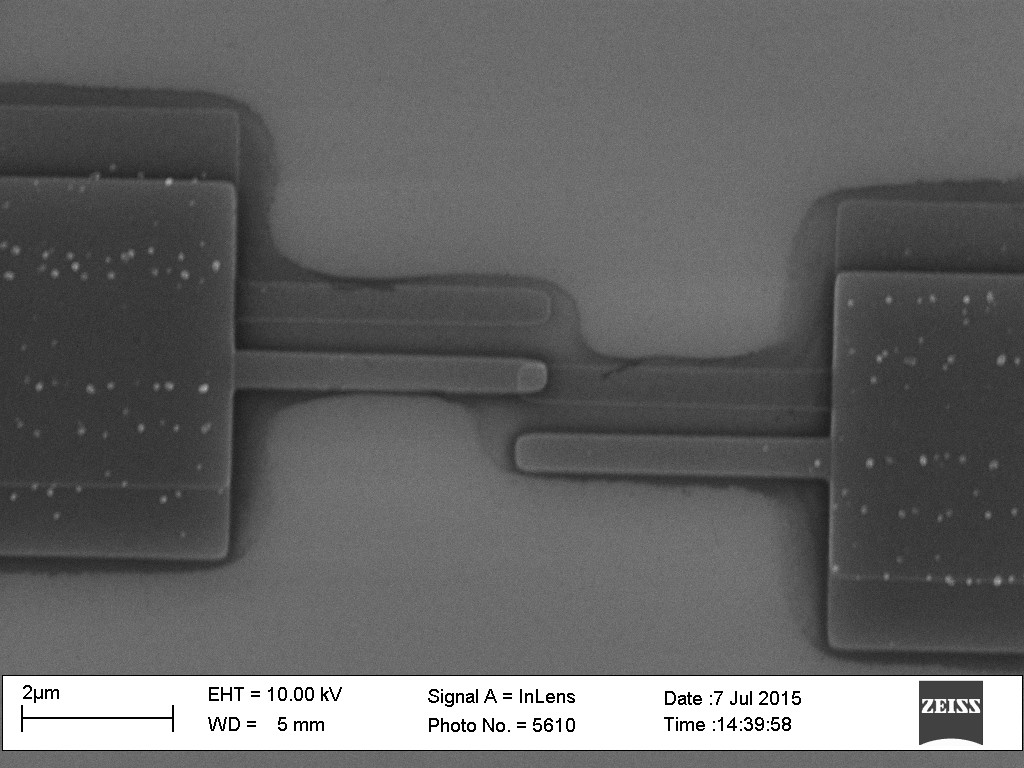
\includegraphics[width=180pt]{SEMexemple.jpg}
                \caption{SEM image of a sample in normal mode}
                \label{SEMexemple}
                \end{subfigure}
                ~
                \begin{subfigure}[t]{0.48\textwidth}
                \centering
                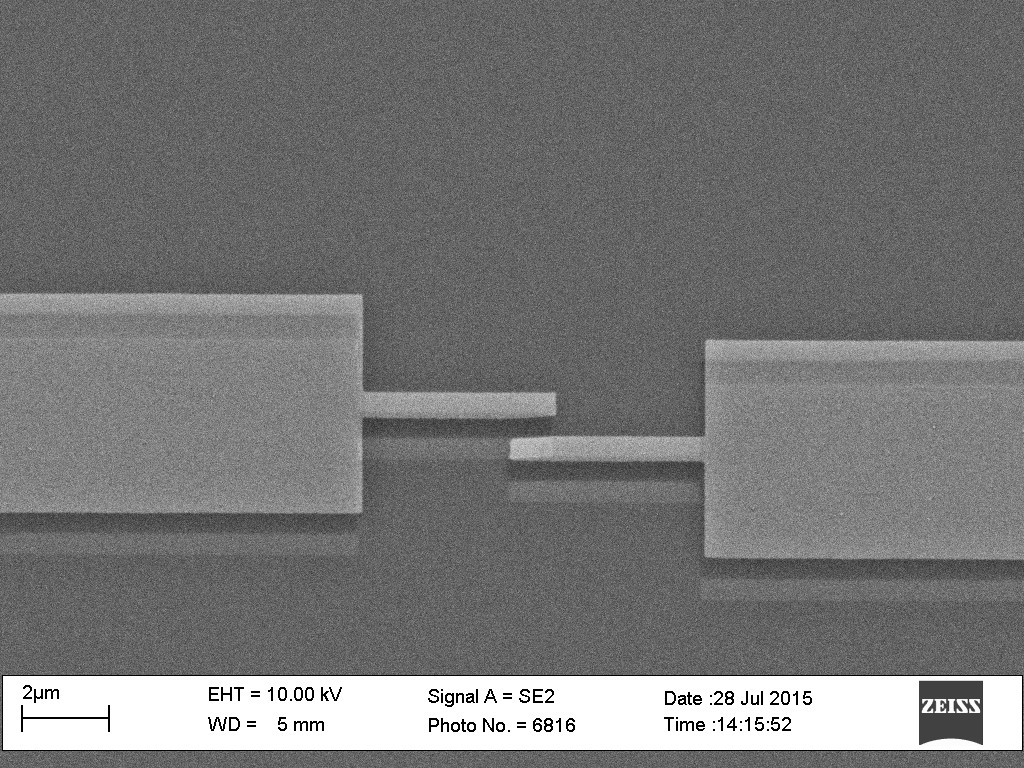
\includegraphics[width=180pt]{SEMexemplese2.jpg}
                \caption{SEM image of a sample in secondary electron mode}
                \label{SEMexemplese2}
                \end{subfigure}
                
                \begin{subfigure}[t]{0.99\textwidth}
                \centering
                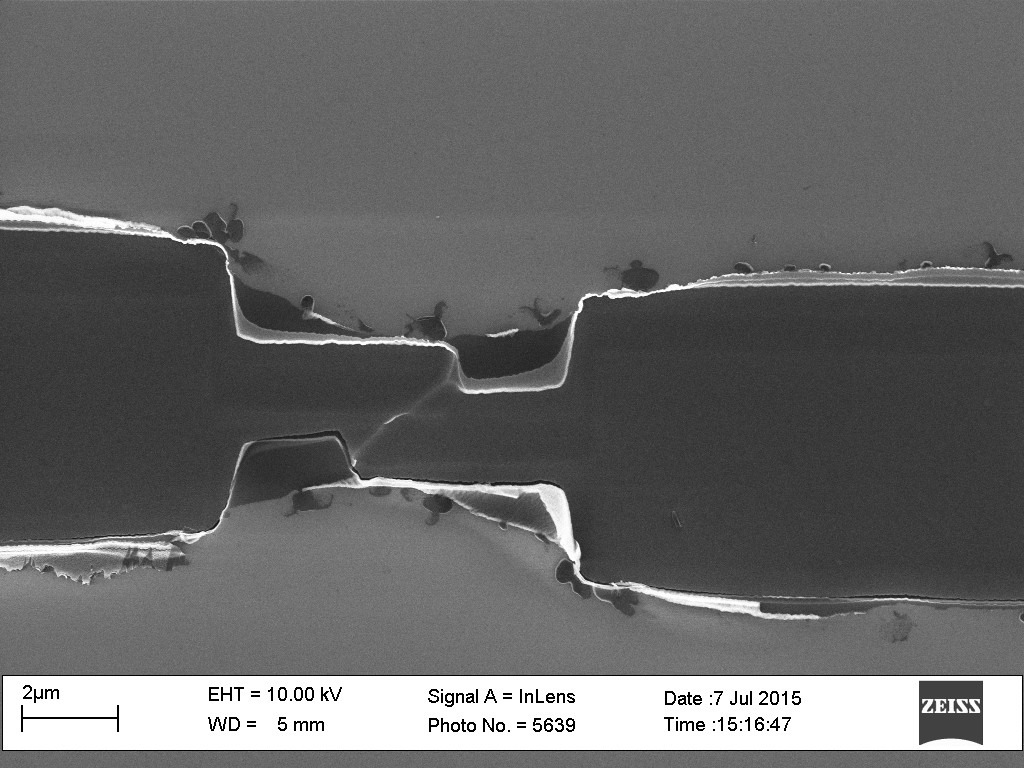
\includegraphics[width=250pt]{SEMexemplefail.jpg}
                \caption{SEM image of a failed sample}
                \label{SEMexemplefail}
                \end{subfigure}
            \end{figure}
            
            
            \section{Dilution cryostat}
            
            \subsection{Cooling theory}    
            The $^4$He is liquid at a temperature of 4.2K. The minimum reachable temperature with $^4$He is 1.2K and 0.3K for the $^3$He by pumping. In order to reach lower temperatures, we use a mixture of $^3$He/$^4$He, where the temperature can be as low as 3mK in the best fridges. The phase diagram of the $^3$He/$^4$He mixture is shown in Fig. \ref{phasediagram} : with 10-15\% of $^3$He, a phase separation will occur below 0.5K due to the existence of a "forbidden zone" in the diagram. We will thus have a rich phase (of $^3$He) and a diluted phase. 
        
        \begin{figure}
            \centering
            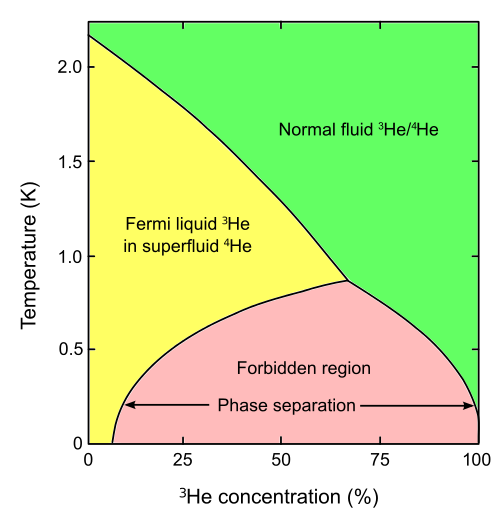
\includegraphics[width=200pt]{phasediagram.png}
            \caption{Phase diagram of $^3$He/$^4$He mixture}
            \label{phasediagram}
        \end{figure}
        
The whole cooling power lies in this phase separation \cite{fridge}. The mixture goes through a 77K nitrogen trap, in order to be cleaned of any impurities, then a line run through the fridge towards the $^4$He bath at 4.2K then to a 1K pot (pumped $^4$He bath). This bath liquefies the mixture which then goes to an exchanger, the still that cools down to 600mK, and ends up in the mixing chamber where the phase separation occurs which has for effect to remove heat from the mixing chamber environment. The mixture is pumped back out of the fridge and injected again through the condensing line, as a close loop.

            \subsection{Preparation of the sample}
            
            The first thing to do with low temperature measurements is to prepare the sample to get in the fridge. Sample holder consists in metallic pads linked to a 12-pins connector. The sample is bounded to the sample holder with thin Al wires with an ultrasound bounder (Fig. \ref{bounding}). The sample holder is screwed to the fridge (Fig. \ref{screwstage}) and sealed in the vacuum chamber (IVC). 
               
               \begin{figure}
                    \centering
                    \begin{subfigure}[t]{0.48\textwidth}
                    \centering
                    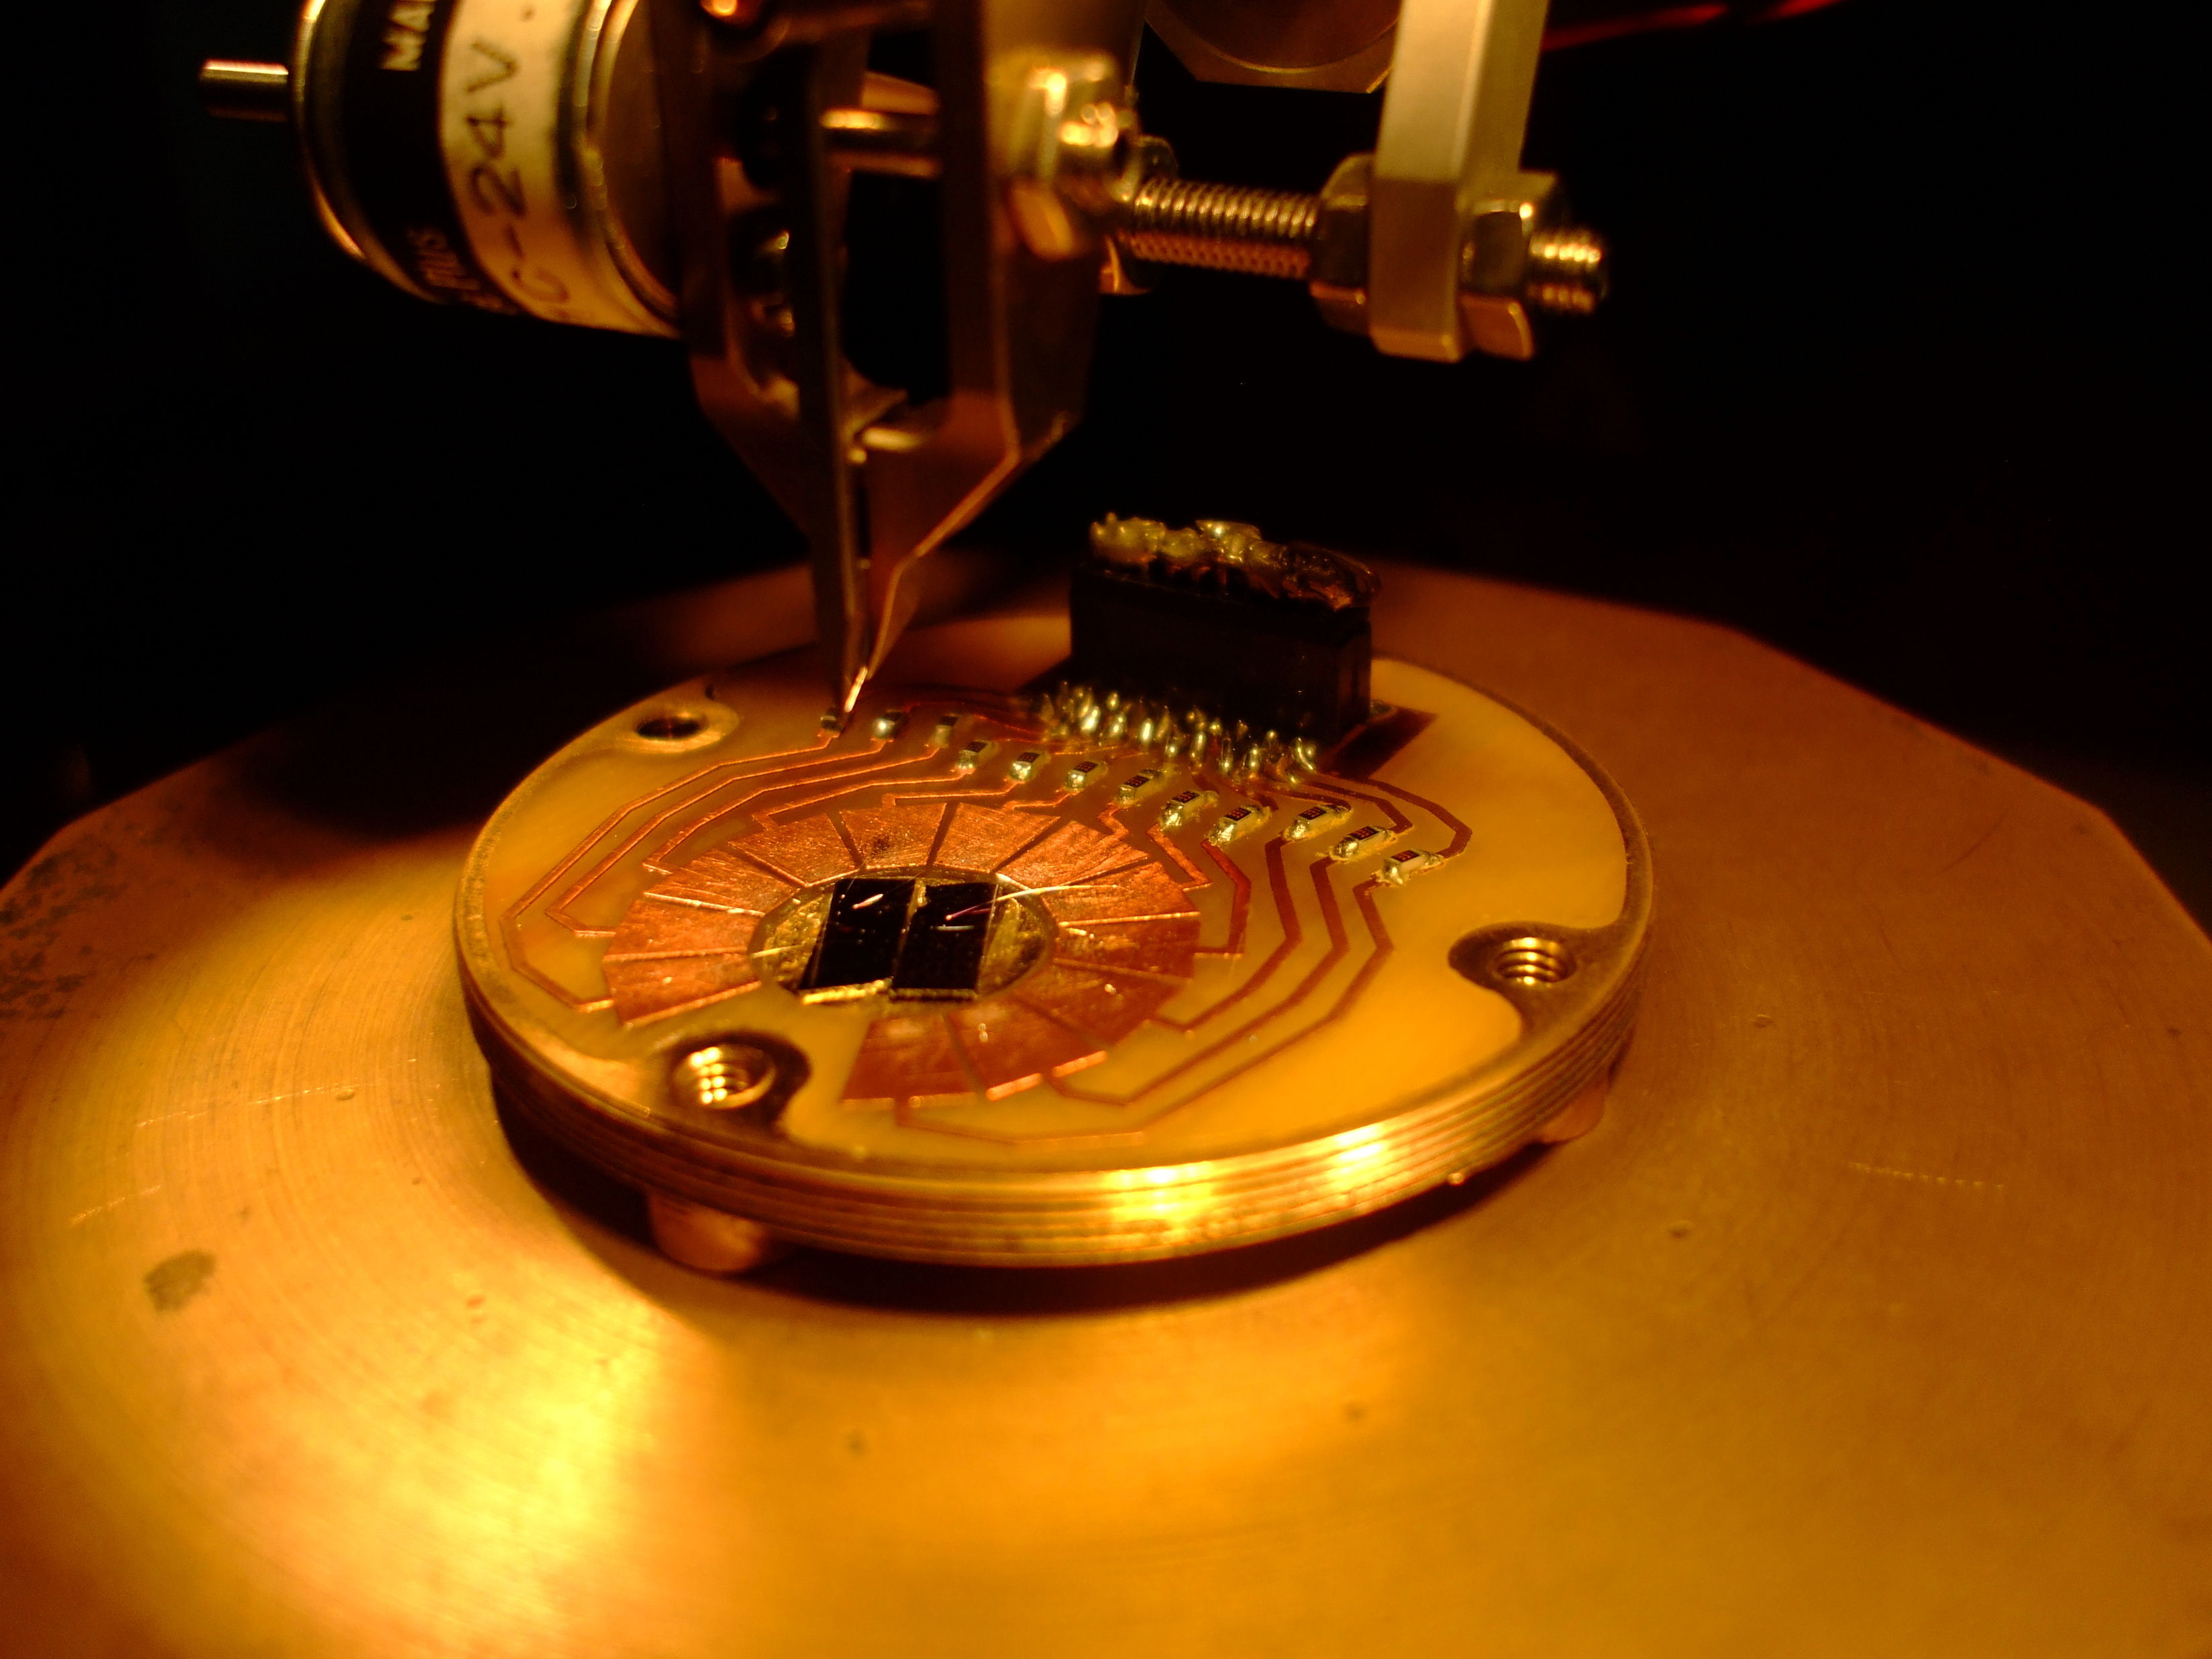
\includegraphics[width=6cm]{bounding.JPG}
                    \caption{Picture of the sample stage}
                    \label{bounding}
                    \end{subfigure}  
                    \begin{subfigure}[t]{0.48\textwidth}
                    \centering
                    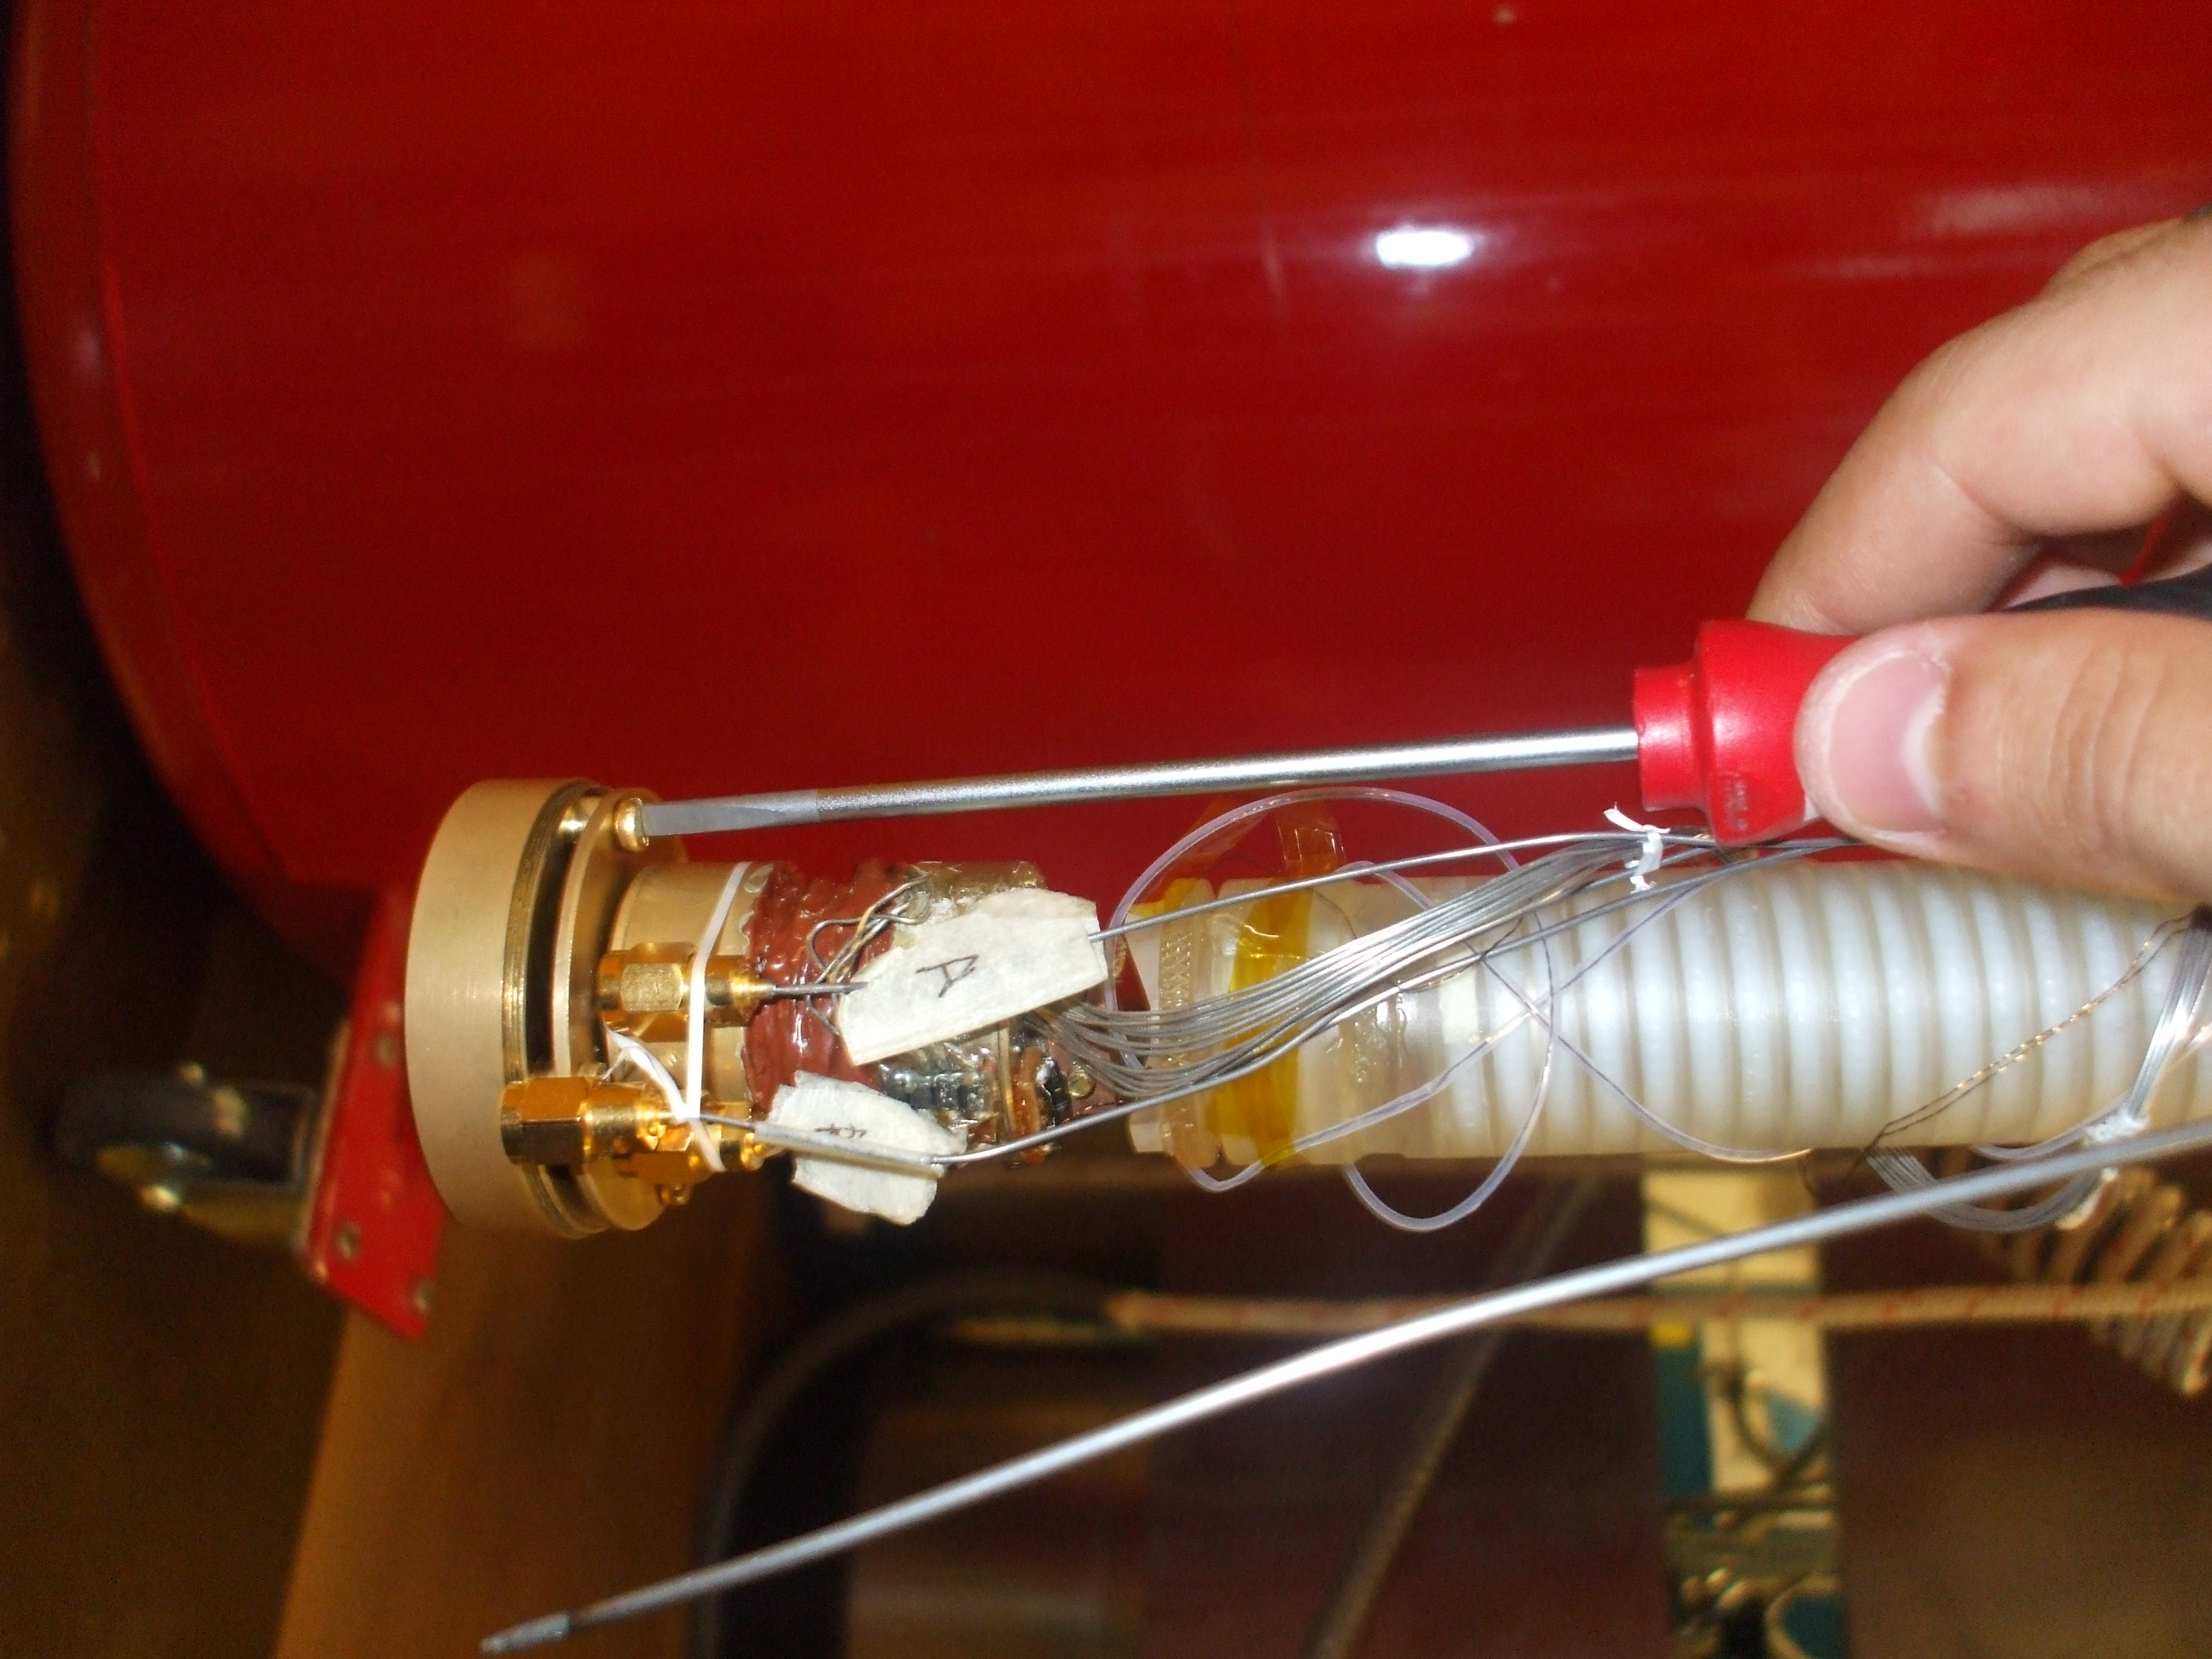
\includegraphics[angle=90,width=5cm]{screwstage.JPG}
                    \caption{Exchanger and mixing chamber with the sample holder}
                    \label{screwstage}
               \end{subfigure}   
               \caption{Pictures of the preparation of the sample stage}         
                \end{figure}
                       
          
            
            \subsection{Cooling down}
            
            The first step of the cooling is to pump the Isolated Vacuum Chamber (IVC) to remove all the air from it and avoid any freezing. Then, some exchange gas (Helium) is inserted into the dilution, in order to reduce the thermal conductivity that exists between the stages of the fridge. The gas will cool down the dilution by convection. The fridge is then placed in a nitrogen bath (Fig. \ref{nitrogen}) during approximatively thirty minutes before diving it in the Helium dewar. The goal is to avoid to evaporate Helium in the dewar (the difference between 77K and 4K is less important and Nitrogen can be cooled more easily). Once the fridge is thermalized at 4K (Fig. \ref{Setup4K}), checked by RuO$_2$ thermoresistor, the exchange gas is pumped back to avoid heat transfert by convection, otherwise the fridge can not be cooled down to 50mK. Finally, the mixture is inserted in the fridge and starts to circulate, like in Fig. \ref{loopmixture}
            
            
            \begin{figure}
            \begin{subfigure}[t]{0.48\textwidth}
            \centering
                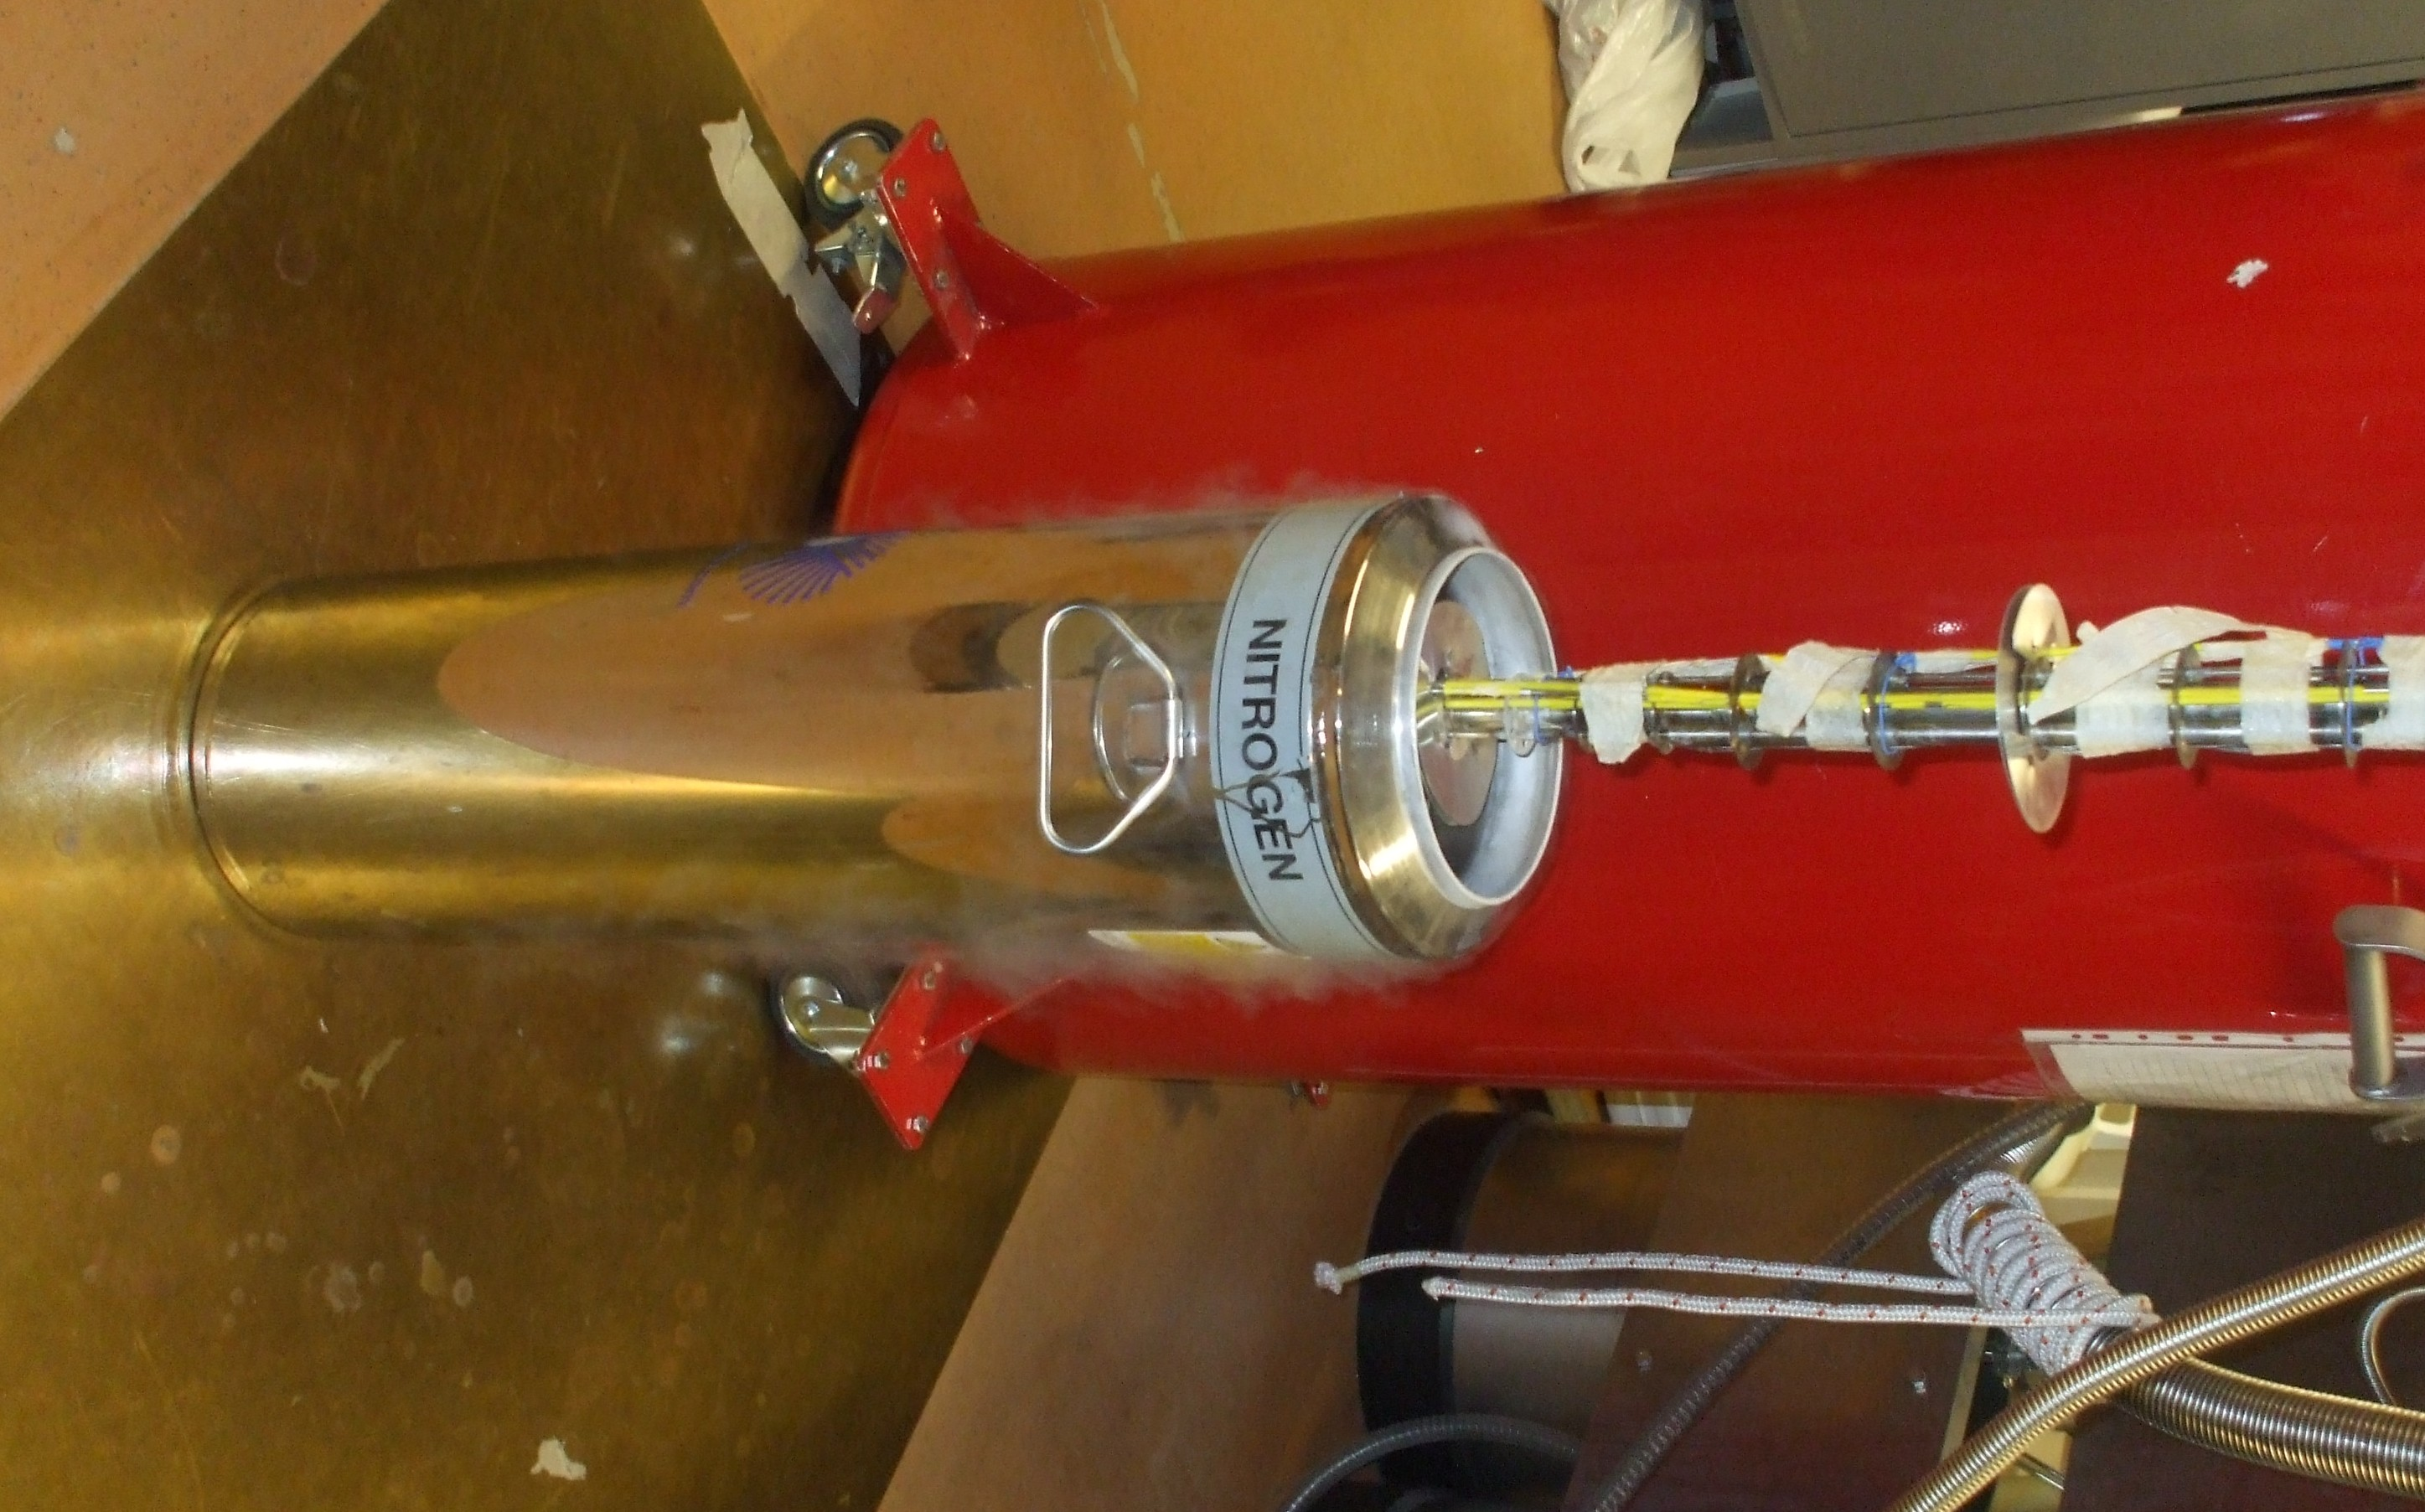
\includegraphics[angle=90,width=4.5cm]{nitrogen.JPG}
                \caption{Picture of the IVC dived into liquid nitrogen}
                \label{nitrogen}
            \end{subfigure}
             \begin{subfigure}[t]{0.48\textwidth}
             \centering
                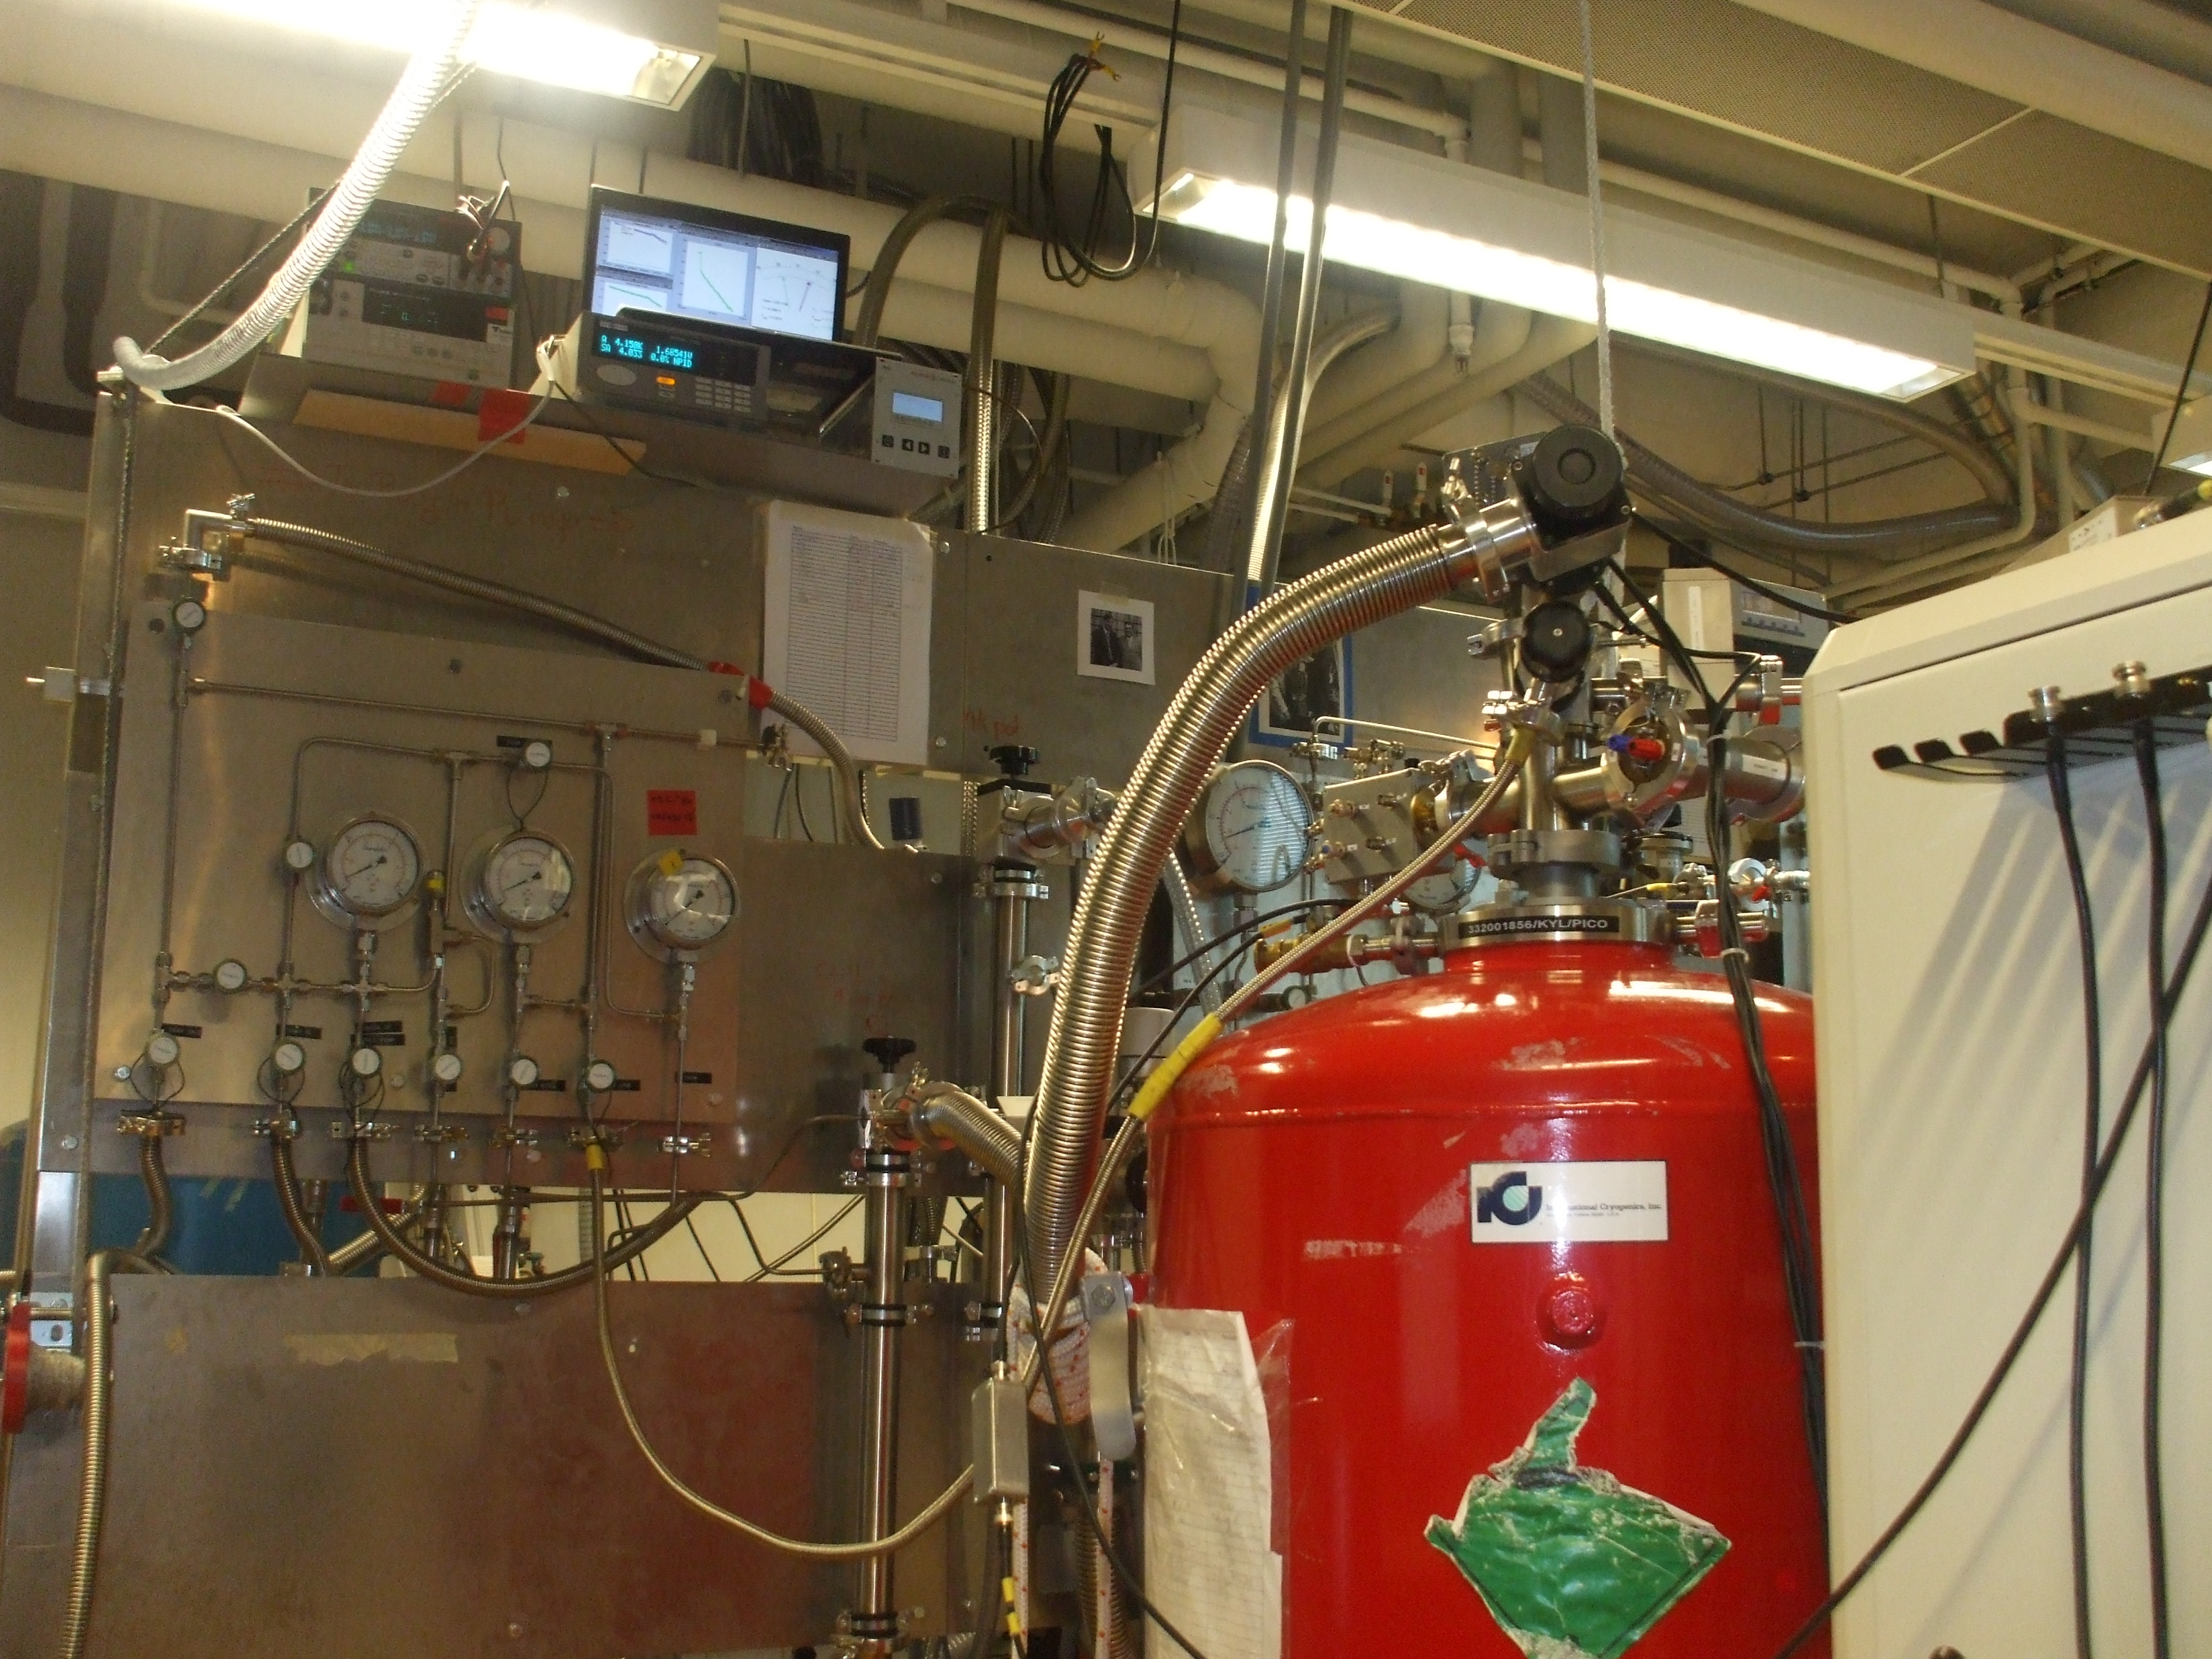
\includegraphics[width=6.4cm]{setup4K.JPG}
                \caption{Picture of the setup when the fridge thermalize at 4.2K}
                \label{Setup4K}
            \end{subfigure}
            \caption{Pictures of the cool down}
            \end{figure}
            
            %After having waited enough, we stop pumping the IVC and we will start to condense. The pressure in the IVC is very low, we stop pumping it and remove the line. We open the 1K pot valves to put some Helium in and pump over it to cool it down to 1K. Since Helium is superfluid at this temperature, we would notice it there was any leak, because it could go everywhere. We put the trap in liquid nitrogen, so that we can flush the condensing and the still lines with mixture. The mixture goes from the pump to the lines through the trap and back to the pump, so it cleans the gas inside the lines : if there was still some air for example. We flush three times to divide the amount of impurities by 10$^8$ (10$^2$ each time). Once the lines are clean, we start to send the mixture to the cryostat through the still line. The still pump contains some mixture, but the tank contains a much larger amount, so we have to open the tank valves to take the mixture from here too. Then we wait until the tak is empty. Once it is empty, and that the temperature is low, we can start to circulate : we close the tank valve and  create a loop for the mixture (See Fig.\ref{loopmixture}), so that it is always moving and cools down the fridge.
            
            \begin{figure}
                \centering
                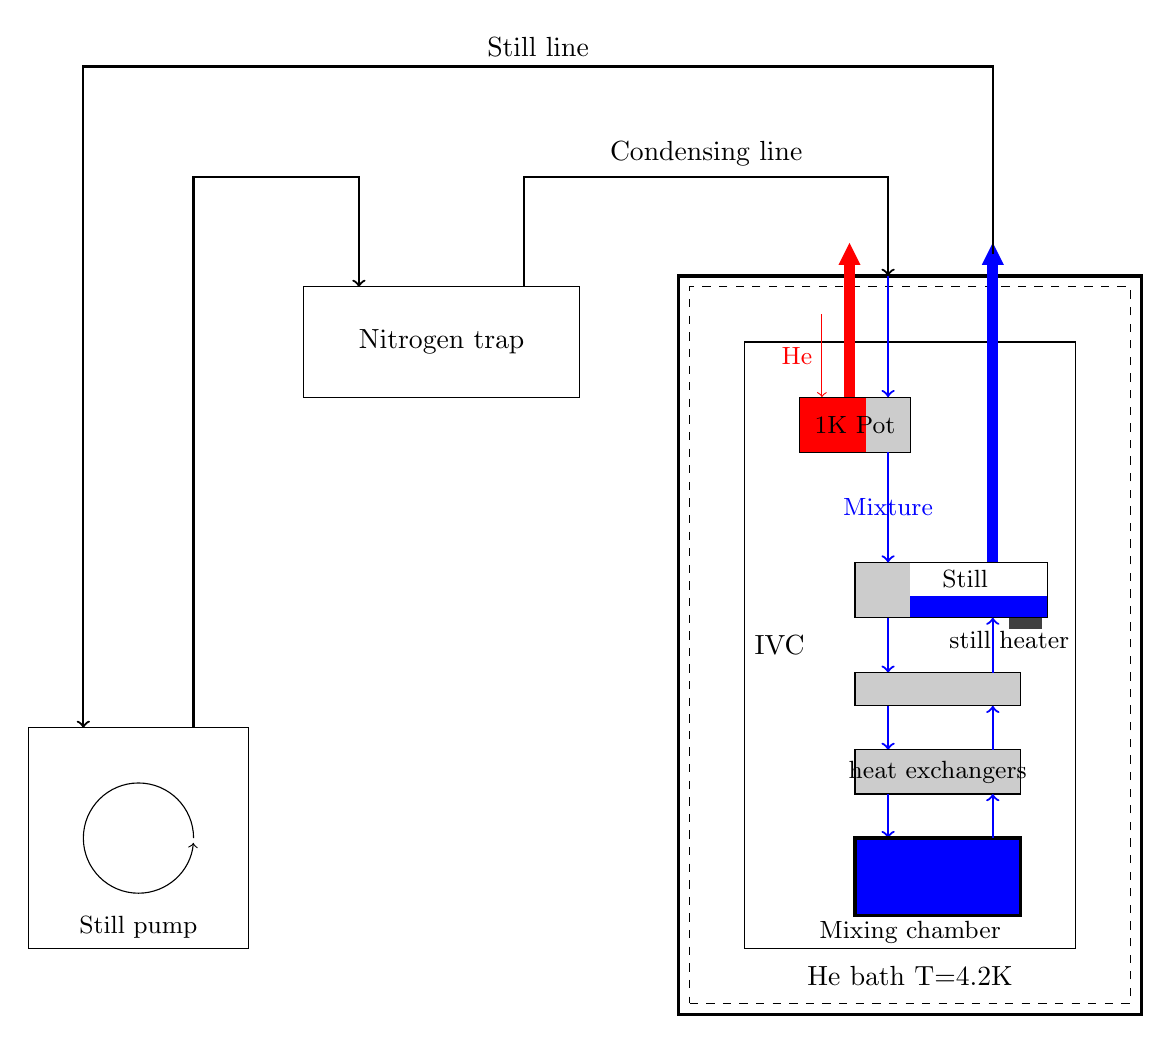
\begin{tikzpicture}[scale=1.4]

\draw (0,2)--(0,4)--(2,4)--(2,2)--cycle;
\draw [->](1.5,3) arc(0:355:0.5);
\draw (1,2)node[above]{{\small Still pump}};

\draw [thick,->](1.5,4)--(1.5,9)--(3,9)--(3,8);
\draw (2.5,8)--(5,8)--(5,7)--(2.5,7)--cycle;
\draw (3.75,7.5)node{Nitrogen trap};
\draw [thick,->] (4.5,8)--(4.5,9)--(7.8,9)node[midway,above]{Condensing line}--(7.8,8.1);

\draw [very thick] (5.9,1.4)--(10.1,1.4)--(10.1,8.1)--(5.9,8.1)--cycle;%HEdewar
\draw (8,1.75)node{He bath T=4.2K};
\draw [dashed] (6,1.5)--(10,1.5)--(10,8)--(6,8)--cycle;
\draw (6.5,2)--(9.5,2)--(9.5,7.5)--(6.5,7.5)--cycle;%IVC
\draw (6.5,4.75)node[right]{IVC};
\fill [color=red] (7,7)--(7.6,7)--(7.6,6.5)--(7,6.5)--cycle;

\draw [color=red,->](7.2,7.75)--(7.2,7)node[midway, left]{{\small He}};
\fill [color=red] (7.4,7)--(7.5,7)--(7.5,8.2)--(7.4,8.2)--cycle;%He
\fill [color=red] (7.35,8.2)--(7.55,8.2)--(7.45,8.4)--cycle;%He
\fill [color=gray!40] (7.6,7)--(7.6,6.5)--(8,6.5)--(8,7)--cycle;%heat exc
\draw (7,7)--(8,7)--(8,6.5)--(7,6.5)--cycle;%1Kpot
\draw (7.5,6.75)node{{\small 1K Pot}};

\draw [color=blue,->, thick](7.8,8.1)--(7.8,7);%mixt
\fill [color=gray!40] (7.5,5.5)--(7.5,5)--(8,5)--(8,5.5)--cycle;
\fill [color=blue] (8,5)--(8,5.2)--(9.25,5.2)--(9.25,5)--cycle;
\draw (7.5,5.5)--(7.5,5)--(9.25,5)--(9.25,5.5)--cycle;%still
\fill [color=gray!150] (8.9,5)--(9.2,5)--(9.2,4.9)--(8.9,4.9)--cycle;
\draw (8.9,4.8)node{{\small still heater}};
\draw [color=blue,->,thick] (7.8,5)--(7.8,4.5); 
\fill [color=gray!40] (7.5,4.5)--(7.5,4.2)--(9,4.2)--(9,4.5)--cycle;

\draw (7.5,4.5)--(7.5,4.2)--(9,4.2)--(9,4.5)--cycle;
\draw [color=blue,->,thick](7.8,4.2)--(7.8,3.8);
\draw (8.5,5.35)node{{\small Still}};
\draw [color=blue,->,thick](7.8,6.5)--(7.8,5.5)node[midway]{{\small Mixture}};%mixt
\fill [color=gray!40] (7.5,3.8)--(7.5,3.4)--(9,3.4)--(9,3.8)--cycle;
\draw (7.5,3.8)--(7.5,3.4)--(9,3.4)--(9,3.8)--cycle;
\draw (8.25,3.6)node{{\small heat exchangers}};
\draw [color=blue,->, thick](7.8,3.4)--(7.8,3);
\fill [color=blue] (7.5,3)--(7.5,2.3)--(9,2.3)--(9,3)--cycle;
\draw [very thick] (7.5,3)--(7.5,2.3)--(9,2.3)--(9,3)--cycle;
\draw (8,2.15)node{{\small Mixing chamber}};
\draw [color=blue,->, thick] (8.75,3)--(8.75,3.4);

\draw [color=blue,->,thick] (8.75,4.5)--(8.75,5);
\draw [color=blue,->,thick] (8.75,3.8)--(8.75,4.2);
\fill [color=blue] (8.7,5.5)--(8.8,5.5)--(8.8,8.2)--(8.7,8.2)--cycle;
\fill [color=blue] (8.65,8.2)--(8.85,8.2)--(8.75,8.4)--cycle;
\draw [->,thick] (8.75,8.3)--(8.75,10)--(0.5,10)node[midway,above]{Still line}--(0.5,4);

\end{tikzpicture}

                \caption[Dilution fridge functioning schematics]{Dilution fridge functioning schematics : The still pump and the nitrogen trap are outside the dewar. The mixture that is injected in the IVC is represented in blue, the $^4$He is in red. The grey parts are heat exchangers}
                \label{loopmixture}
            \end{figure}
            
%             \subsection{Warming up}
%             
%             Warming up the fridge is quite easy, first we have to stop the circulation of the mixture by closing the trap in and start to pump it from both still and condensing lines to the tank, so we open the tank and still valves. The mixture is liquid so it is difficult to pump it in this state. To ease the pumping, we will heat up to evaporate the mixture. For this, there are two lines where we can apply some voltage, which will go through thermoresistor and heat the area and then the mixture. Since the mixture is pump with the still pump, we have to be careful that the pressure does not exceed 1 mbar, or it could damage the pump. To avoid huge augmentation of the pressure we increase slowly the applied voltage, especially around 1.3K when the mixture starts to boil. Of course, we can control the temperature through Matlab, like we did for the cool down. The pressure increases while the mixture is evaporated. It can take one hour until the mixture is totally pumped out.
%             
%             Once it is the case, the temperature increase rapidly and the pressure goes down. Here, we wait five minutes to be sure all the mixture went out. Then, we close all the valves of the condensing line and the still line, we keep pumping the mixture to the tank, finally, we close the tank and remove the fridge from the dewar. Here, the fridge just needs to thermalize at the room temperature, we let it like that for a while before removing the sample and getting the fridge ready for the next cooling.
%             
%             
